\documentclass[11pt,letterpaper]{article}
\usepackage[utf8]{inputenc}
\usepackage[T1]{fontenc}
\usepackage[margin=2.4cm]{geometry}
\usepackage{hyperref}
\usepackage{verbatim}
\usepackage{parskip}
\usepackage{graphicx}

\hypersetup{colorlinks=true, linkcolor=blue, urlcolor=blue}

\title{\textbf{Actividad 4: Docker, Docker Compose y microservicios}\\[0.3em]
\large Adaptaci\'on del pipeline de scikit-learn a una arquitectura de contenedores}
\author{Diego Linares \and Andy Fuentes \and Diederich Solis \and Christian Echeverria}
\date{Machine Learning Engineering (MLE/MLOps) --- Universidad del Valle de Guatemala\\
Agosto 2026}

\begin{document}
\maketitle

\begin{center}
\textbf{Repositorio:} \url{https://github.com/DiegoLinares11/Actividad4-MLOPS}
\end{center}

\hrule
\vspace{1em}

\section{Introducci\'on: el problema que motiva todo}

En la Actividad 3 calibramos los hiperpar\'ametros de un pipeline de scikit-learn sobre el dataset
de la UEFA Champions League. Al ejecutarlo en dos computadoras distintas nos encontramos con algo
revelador: \textbf{el mismo c\'odigo, con la misma semilla \texttt{random\_state=42}, dio puntajes
distintos}. En Windows, \texttt{GridSearchCV} report\'o un \texttt{f1\_macro} de 0.563; en macOS,
0.611. La causa no era el azar sino que cada m\'aquina ten\'ia una versi\'on distinta de
scikit-learn instalada.

Ese hallazgo es exactamente el problema que Docker resuelve: \textbf{empaquetar la aplicaci\'on
junto con su sistema operativo, sus librer\'ias y sus versiones exactas}, de modo que se ejecute
de forma id\'entica en cualquier m\'aquina. Fijar la semilla no alcanza para reproducir un
experimento; hay que fijar tambi\'en el entorno completo.

\section{Docker}

\subsection{Contenedores frente a m\'aquinas virtuales}

Un contenedor \textbf{no} es una m\'aquina virtual peque\~na. Es un proceso normal del sistema
anfitri\'on, aislado mediante funciones del kernel de Linux: los \emph{namespaces} hacen que el
proceso vea su propio sistema de archivos, su propia red y su propia tabla de procesos, mientras
que los \emph{cgroups} limitan cu\'anta CPU y memoria puede consumir.

\begin{center}
\begin{tabular}{|l|l|l|}
\hline
& \textbf{M\'aquina virtual} & \textbf{Contenedor} \\
\hline
Qu\'e virtualiza & El hardware completo & Solo el proceso \\
Sistema operativo & Cada VM lleva el suyo entero & Comparten el kernel del anfitri\'on \\
Tama\~no t\'ipico & Gigabytes & Decenas o cientos de MB \\
Tiempo de arranque & Minutos & Segundos \\
Aislamiento & Total & A nivel de proceso \\
\hline
\end{tabular}
\end{center}

La consecuencia pr\'actica es que en una laptop se pueden correr decenas de contenedores, pero
apenas dos o tres m\'aquinas virtuales.

\subsection{Dockerfile, imagen y contenedor}

Son tres conceptos que conviene no confundir:

\begin{center}
\begin{tabular}{|l|l|l|}
\hline
\textbf{Concepto} & \textbf{Qu\'e es} & \textbf{Analog\'ia} \\
\hline
Dockerfile & La receta: instrucciones para construir & El plano de una casa \\
Imagen & El resultado, inmutable y de solo lectura & La casa construida \\
Contenedor & Una imagen en ejecuci\'on & La casa habitada \\
\hline
\end{tabular}
\end{center}

De una misma imagen se pueden levantar muchos contenedores. La imagen \textbf{nunca cambia}: lo
que un contenedor escribe va a una capa temporal por encima, que \textbf{se elimina junto con el
contenedor}. De esa propiedad se desprende toda la discusi\'on sobre persistencia de la
secci\'on~\ref{sec:volumenes}.

\subsection{Capas y cach\'e de construcci\'on}

Cada instrucci\'on del Dockerfile genera una \textbf{capa}, y Docker las almacena en cach\'e: si
una capa no cambi\'o respecto a la construcci\'on anterior, se reutiliza. Por eso en nuestros
Dockerfiles las dependencias se copian e instalan \textbf{antes} que el c\'odigo:

\begin{verbatim}
COPY entrenador/requirements.txt ./requirements.txt   # cambia poco -> capa cacheada
RUN pip install --no-cache-dir -r requirements.txt    # la instruccion lenta
COPY entrenador/entrenar.py ./                        # cambia mucho -> capa barata
\end{verbatim}

Con el orden invertido, modificar una sola l\'inea del script obligar\'ia a reinstalar
scikit-learn completo en cada construcci\'on.

\subsection{Comandos fundamentales}

\begin{verbatim}
docker build -t mi-imagen .      # construir una imagen desde el Dockerfile
docker images                    # listar imagenes
docker run mi-imagen             # levantar un contenedor
docker ps                        # contenedores corriendo (-a incluye detenidos)
docker logs <contenedor>         # ver su salida
docker exec -it <contenedor> sh  # abrir una terminal adentro
docker rm / docker rmi           # eliminar contenedor / imagen
\end{verbatim}

\section{Docker Compose}

Docker administra un contenedor a la vez. Nuestra aplicaci\'on tiene tres, con dependencias
reales entre ellos: la API no sirve de nada si el modelo todav\'ia no existe, y no puede guardar
nada si la base de datos a\'un no arranc\'o.

Docker Compose describe \textbf{el sistema completo en un archivo YAML} y lo levanta en el orden
correcto con un solo comando:

\begin{verbatim}
docker compose up --build   # construir y levantar todo
docker compose ps           # estado de cada servicio
docker compose logs -f api  # seguir los logs de un servicio
docker compose down         # apagar y borrar contenedores (los volumenes SE QUEDAN)
docker compose down -v      # apagar y borrar TAMBIEN los volumenes (destructivo)
\end{verbatim}

Adem\'as de la comodidad, Compose aporta cuatro cosas que tendr\'iamos que resolver a mano:

\begin{enumerate}
\item \textbf{Red privada autom\'atica.} Compose crea una red y los servicios se localizan por
\emph{nombre}: la API se conecta a \texttt{postgresql://...@db:5432/...}, literalmente
\texttt{db}, sin necesidad de direcciones IP. Docker ejecuta un DNS interno.

\item \textbf{Orden de arranque real.} Mediante \texttt{depends\_on} con condiciones:
\texttt{service\_completed\_successfully} hace que la API espere a que el entrenador
\emph{termine correctamente}, y \texttt{service\_healthy} la hace esperar a que Postgres pase su
\texttt{healthcheck}. Esto sustituye al t\'ipico ``esperar cinco segundos y confiar''.

\item \textbf{Configuraci\'on por variables de entorno}, le\'idas de un archivo \texttt{.env} que
no se versiona en el repositorio.

\item \textbf{Aislamiento hacia el exterior.} Solo la API publica un puerto; Postgres es
inalcanzable desde fuera aunque los contenedores s\'i lo vean entre ellos.
\end{enumerate}

\section{Adaptaci\'on del pipeline a microservicios}

\subsection{Por qu\'e separar}

En la Actividad 3 todo era un \'unico programa que le\'ia el CSV, calibraba, evaluaba e imprim\'ia
resultados. Eso funciona en una laptop, pero no en producci\'on: entrenar tarda minutos y consume
CPU, mientras que responder una predicci\'on debe tardar milisegundos. Si ambas tareas comparten
proceso, cada reentrenamiento deja la aplicaci\'on sin responder.

\subsection{Los tres servicios}

\begin{center}
\begin{tabular}{|l|l|p{5.2cm}|l|}
\hline
\textbf{Servicio} & \textbf{Tipo} & \textbf{Qu\'e hace} & \textbf{Ciclo de vida} \\
\hline
\texttt{entrenador} & Por lotes & Lee el CSV, calibra con
\texttt{RandomizedSearchCV} y guarda el modelo & Corre y termina \\
\hline
\texttt{api} & Servicio & Carga el modelo del volumen y responde
predicciones por HTTP (FastAPI) & Siempre encendido \\
\hline
\texttt{db} & Estado & Guarda el historial de predicciones
(PostgreSQL) & Siempre encendido \\
\hline
\end{tabular}
\end{center}

El flujo es el siguiente: el \texttt{entrenador} lee el dataset desde un \emph{bind mount} de solo
lectura, calibra los hiperpar\'ametros y escribe \texttt{modelo.joblib} en un volumen compartido;
luego termina y su contenedor muere. La \texttt{api} monta ese mismo volumen en modo solo lectura,
carga el modelo y expone los endpoints \texttt{/salud}, \texttt{/modelo}, \texttt{/predecir} y
\texttt{/predicciones}. Cada predicci\'on se registra en \texttt{db}, que persiste en su propio
volumen.

\subsection{Ventajas concretas de esta separaci\'on}

\begin{itemize}
\item \textbf{Escalado independiente:} ante mucha carga, \texttt{docker compose up --scale api=3}
levanta tres copias de la API sin tocar el entrenador.
\item \textbf{Reentrenar no interrumpe el servicio:} la API sigue sirviendo el modelo anterior
mientras el entrenador produce el nuevo.
\item \textbf{Im\'agenes m\'as peque\~nas y espec\'ificas:} la API no necesita el dataset ni el
c\'odigo de calibraci\'on.
\item \textbf{Fallos aislados:} si Postgres se cae, la API contin\'ua prediciendo y \'unicamente
deja de registrar el historial.
\end{itemize}

\subsection{El detalle t\'ecnico que hace posible todo esto}

El modelo se serializa con \texttt{joblib}, y un objeto serializado \textbf{guarda la ruta de
importaci\'on de sus clases, no su c\'odigo}. Nuestro pipeline contiene los transformadores
\texttt{PorcentajeATexto} y \texttt{RatioATexto}, que son clases propias. Si la API no pudiera
importarlas desde el mismo m\'odulo, la carga del modelo fallar\'ia.

Por ese motivo \textbf{ambas im\'agenes instalan el mismo paquete}
(\texttt{act3\_pipeline-0.1.0-py3-none-any.whl}) que empaquetamos en la Actividad 3, y ambos
archivos \texttt{requirements.txt} fijan \textbf{exactamente las mismas versiones} de
scikit-learn, pandas, numpy y scipy. Aqu\'i se ve para qu\'e serv\'ia el trabajo de empaquetado de
la actividad anterior.

\section{Vol\'umenes y persistencia de datos}
\label{sec:volumenes}

\subsection{El problema de fondo}

El sistema de archivos de un contenedor es la imagen (de solo lectura) m\'as una \textbf{capa
escribible} superpuesta. Esa capa pertenece al contenedor: al eliminarlo, se elimina con \'el.

Si el entrenador guardara el modelo en \texttt{/app/modelo.joblib}, al terminar el contenedor el
modelo desaparecer\'ia y la API nunca lo ver\'ia. Si Postgres escribiera su base en la capa
escribible, cada \texttt{docker compose down} borrar\'ia el historial completo.

\subsection{Las cuatro formas de manejar datos}

\begin{center}
\begin{tabular}{|l|p{3.6cm}|l|p{4cm}|}
\hline
\textbf{Forma} & \textbf{D\'onde vive} & \textbf{Sobrevive} & \textbf{Cu\'ando usarla} \\
\hline
Capa escribible & Dentro del contenedor & No & Archivos temporales \\
\hline
Volumen con nombre & \'Area administrada por Docker & S\'i & Datos de la aplicaci\'on: bases de
datos, modelos \\
\hline
Bind mount & Una carpeta del anfitri\'on & S\'i & C\'odigo, datos de entrada, configuraci\'on \\
\hline
tmpfs & Memoria RAM & Nunca toca disco & Secretos y temporales \\
\hline
\end{tabular}
\end{center}

En este proyecto usamos las dos intermedias:

\begin{verbatim}
volumes:
  - ./datos:/datos:ro      # BIND MOUNT: carpeta del anfitrion, de solo lectura
  - modelos:/modelos       # VOLUMEN CON NOMBRE: lo administra Docker
\end{verbatim}

\subsection{Volumen con nombre frente a bind mount}

\begin{center}
\begin{tabular}{|l|l|l|}
\hline
& \textbf{Volumen con nombre} & \textbf{Bind mount} \\
\hline
Lo administra & Docker & El usuario \\
Ruta & Irrelevante para el usuario & Depende de cada m\'aquina \\
Portabilidad & Alta & Baja \\
Rendimiento (Docker Desktop) & Mejor & Peor \\
Ideal para & Bases de datos, modelos & C\'odigo, datos de entrada \\
\hline
\end{tabular}
\end{center}

La regla pr\'actica es simple: \textbf{si lo produce la aplicaci\'on, volumen con nombre; si lo
escribe el desarrollador, bind mount}.

\subsection{Por qu\'e el modelo no va dentro de la imagen}

Ser\'ia tentador entrenar durante la construcci\'on de la imagen y dejar el modelo incorporado. Es
una mala pr\'actica por tres razones:

\begin{enumerate}
\item Reentrenar obligar\'ia a reconstruir y redistribuir la imagen completa.
\item Las im\'agenes deben ser inmutables y reproducibles; entrenar durante la construcci\'on las
vuelve dependientes de los datos del momento.
\item El modelo es \textbf{estado}, no c\'odigo, y se versiona de manera distinta.
\end{enumerate}

\subsection{Comandos de vol\'umenes}

\begin{verbatim}
docker volume ls                                # listar
docker volume inspect actividad4-mlops_modelos  # ver donde vive realmente
docker volume rm <nombre>                       # eliminar (destructivo)
docker volume prune                             # eliminar los que nadie usa
\end{verbatim}

\subsection{Un problema real: permisos y vol\'umenes}

Al levantar el sistema por primera vez, el entrenamiento se complet\'o correctamente pero el
guardado fall\'o:

\begin{verbatim}
[entrenador] listo en 12.0 s | mejor f1_macro en CV = 0.619
[entrenador] modelo final: LogisticRegression
PermissionError: [Errno 13] Permission denied: '/modelos/modelo.joblib'
\end{verbatim}

La causa es la interacci\'on entre dos buenas pr\'acticas que chocan entre s\'i. Por seguridad, el
contenedor no corre como \texttt{root} sino como un usuario sin privilegios
(\texttt{mlops}, uid 1000). Pero cuando Docker monta un volumen con nombre que est\'a vac\'io,
\textbf{copia el propietario y los permisos de esa carpeta tal como existe en la imagen}; si la
carpeta no existe en la imagen, el volumen se crea perteneciendo a \texttt{root} y el usuario sin
privilegios no puede escribir en \'el.

La soluci\'on es crear el directorio dentro de la imagen y asignarle el propietario correcto
\emph{antes} de que el volumen se monte encima:

\begin{verbatim}
RUN useradd --create-home --uid 1000 mlops \
    && mkdir -p /modelos \
    && chown -R mlops:mlops /app /modelos
USER mlops
\end{verbatim}

Como el volumen ya se hab\'ia creado con el propietario equivocado, hubo que eliminarlo con
\texttt{docker compose down -v} para que naciera de nuevo con los permisos correctos. Es un error
frecuente y vale la pena registrarlo: el volumen recuerda su propietario igual que recuerda sus
datos.

\subsection{Demostraci\'on de la persistencia}

Las tres pruebas se ejecutaron sobre el sistema ya funcionando. Estos son los resultados reales.

\textbf{Prueba 1: el modelo sobrevive a su creador.}

\begin{verbatim}
SERVICE      STATE     STATUS
api          running   Up 15 seconds (healthy)
db           running   Up 32 seconds (healthy)
entrenador   exited    Exited (0) 15 seconds ago

$ curl http://localhost:8000/salud
{"estado":"ok","contenedor":"72e91038c58f","modelo_cargado":true,"base_de_datos":true}
\end{verbatim}

El contenedor \texttt{act4-entrenador} ya termin\'o, y sin embargo la API tiene el modelo cargado
y responde. Los metadatos indican que lo entren\'o el contenedor \texttt{3e635acd60eb}, que ya no
existe.

Con el modelo en servicio, dos predicciones sobre partidos del propio dataset:

\begin{verbatim}
Real Madrid vs Marseille (resultado real 2-1):
  {"prediccion": "Home Win",
   "probabilidades": {"Home Win": 0.8764, "Draw": 0.1185, "Away Win": 0.0051}}

Ajax vs Inter (resultado real 0-2):
  {"prediccion": "Away Win",
   "probabilidades": {"Away Win": 0.7822, "Draw": 0.1868, "Home Win": 0.0310}}
\end{verbatim}

\textbf{Prueba 2: la base sobrevive a un apagado completo.} Tras \texttt{docker compose down},
\texttt{docker compose ps -a} no lista ning\'un contenedor, pero \texttt{docker volume ls} sigue
mostrando \texttt{actividad4-mlops\_modelos} y \texttt{actividad4-mlops\_pgdata}. Al levantar de
nuevo con \texttt{docker compose up -d}:

\begin{verbatim}
[entrenador] contenedor 8910543744d3 | python 3.12.14 | sklearn 1.8.0
[entrenador] ya existe /modelos/modelo.joblib (viene del volumen de una corrida anterior)
[entrenador] no se reentrena. Para forzarlo: FORZAR_REENTRENO=1

$ curl http://localhost:8000/predicciones
{"total_historico": 2, ...}

entrenado_en: 2026-08-19T02:44:37+00:00
contenedor que lo entreno: 3e635acd60eb
\end{verbatim}

El entrenador es un contenedor \emph{nuevo} (\texttt{8910543744d3}) que encontr\'o el trabajo del
anterior y decidi\'o no repetirlo; las dos predicciones siguen en la base; y los metadatos del
modelo siguen apuntando al contenedor original. Nada de eso sobrevivir\'ia sin vol\'umenes.

\textbf{Prueba 3: sin vol\'umenes no queda nada.} Con \texttt{docker compose down -v}:

\begin{verbatim}
Volume actividad4-mlops_modelos Removed
Volume actividad4-mlops_pgdata  Removed

$ docker volume ls --filter name=actividad4
DRIVER    VOLUME NAME
(vacio)
\end{verbatim}

Al levantar otra vez, el entrenador vuelve a trabajar desde cero y el historial se pierde:

\begin{verbatim}
[entrenador] calibrando con RandomizedSearchCV, 60 combinaciones, metrica f1_macro...
[entrenador] listo en 14.9 s | mejor f1_macro en CV = 0.619
[entrenador] modelo guardado en /modelos/modelo.joblib (10 KB)

$ curl http://localhost:8000/predicciones
{"total_historico": 0, "predicciones": []}
\end{verbatim}

Esa es exactamente la diferencia entre \texttt{down} y \texttt{down -v}, y la raz\'on por la que
la segunda se escribe con cuidado.

\subsection{Comprobaci\'on de reproducibilidad}

El resultado m\'as importante de toda la actividad es este: el modelo entrenado \textbf{dentro del
contenedor} dio exactamente los mismos n\'umeros que en las dos computadoras de la Actividad 3.

\begin{center}
\begin{tabular}{|l|l|l|l|}
\hline
& \textbf{Windows (Act.\ 3)} & \textbf{macOS (Act.\ 3)} & \textbf{Contenedor (Act.\ 4)} \\
\hline
Modelo ganador & LogisticRegression & LogisticRegression & LogisticRegression \\
\texttt{f1\_macro} en CV & 0.619 & 0.619 & 0.619 \\
Accuracy en test & 0.690 & 0.690 & 0.690 \\
\texttt{f1\_macro} en test & 0.631 & 0.631 & 0.631 \\
\hline
\end{tabular}
\end{center}

La diferencia respecto a la Actividad 3 es la garant\'ia. All\'a los n\'umeros coincidieron por
suerte: la discrepancia en los puntajes de las b\'usquedas basadas en Random Forest (0.563 contra
0.611) mostraba que las dos m\'aquinas no estaban ejecutando lo mismo. Aqu\'i la imagen fija
scikit-learn 1.8.0, pandas 2.3.3 y Python 3.12.14, as\'i que cualquier computadora que levante el
contenedor ejecuta \emph{exactamente} el mismo entorno. La causa del problema queda eliminada de
ra\'iz, no solo su s\'intoma.

\emph{Nota:} el servicio entrenador ejecuta \'unicamente \texttt{RandomizedSearchCV}, que fue la
b\'usqueda ganadora en la Actividad 3; no se volvieron a medir dentro del contenedor las otras dos
b\'usquedas.

\section{Evidencia de ejecuci\'on}

Las capturas completas est\'an en la carpeta \texttt{capturas/} del repositorio. Se incluyen aqu\'i
las cuatro m\'as representativas.

\begin{figure}[ht]
\centering
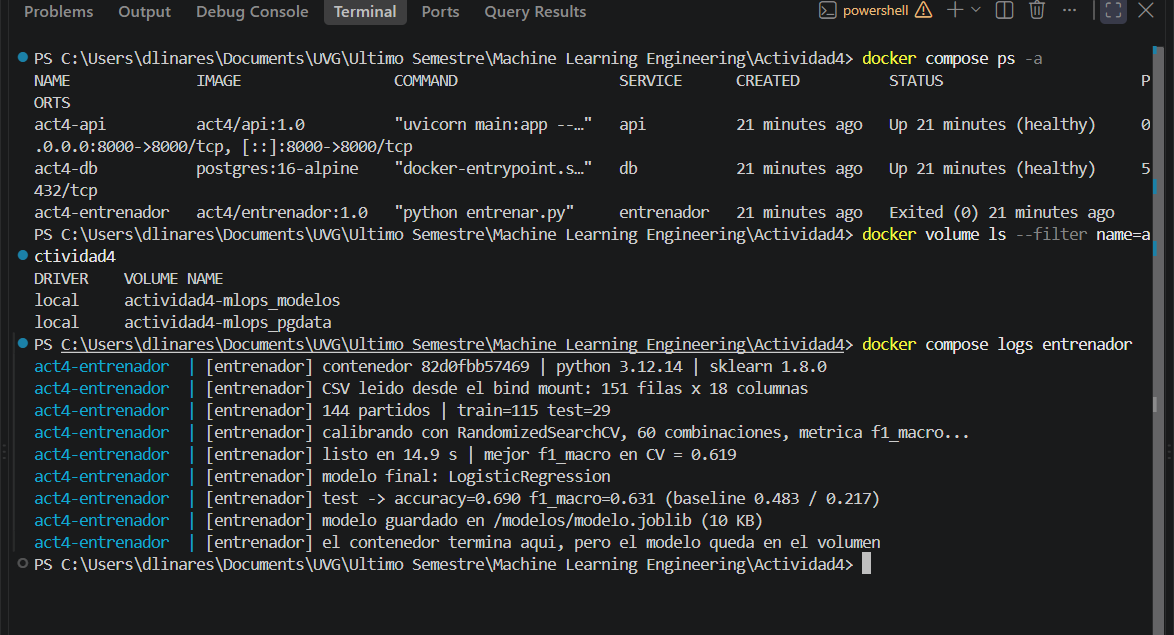
\includegraphics[width=\textwidth]{capturas/entrenamientoTerminal.png}
\caption{Tres comandos en una sola vista. Arriba, \texttt{docker compose ps -a}: la API y la base
en \emph{Up (healthy)} y el entrenador en \emph{Exited (0)}. En medio, \texttt{docker volume ls}
con los dos vol\'umenes. Abajo, los registros del entrenador con el resultado del entrenamiento
(\texttt{f1\_macro} en CV de 0.619, \emph{accuracy} de 0.690 en prueba) y la l\'inea final: ``el
contenedor termina aqui, pero el modelo queda en el volumen''.}
\end{figure}

\begin{figure}[ht]
\centering
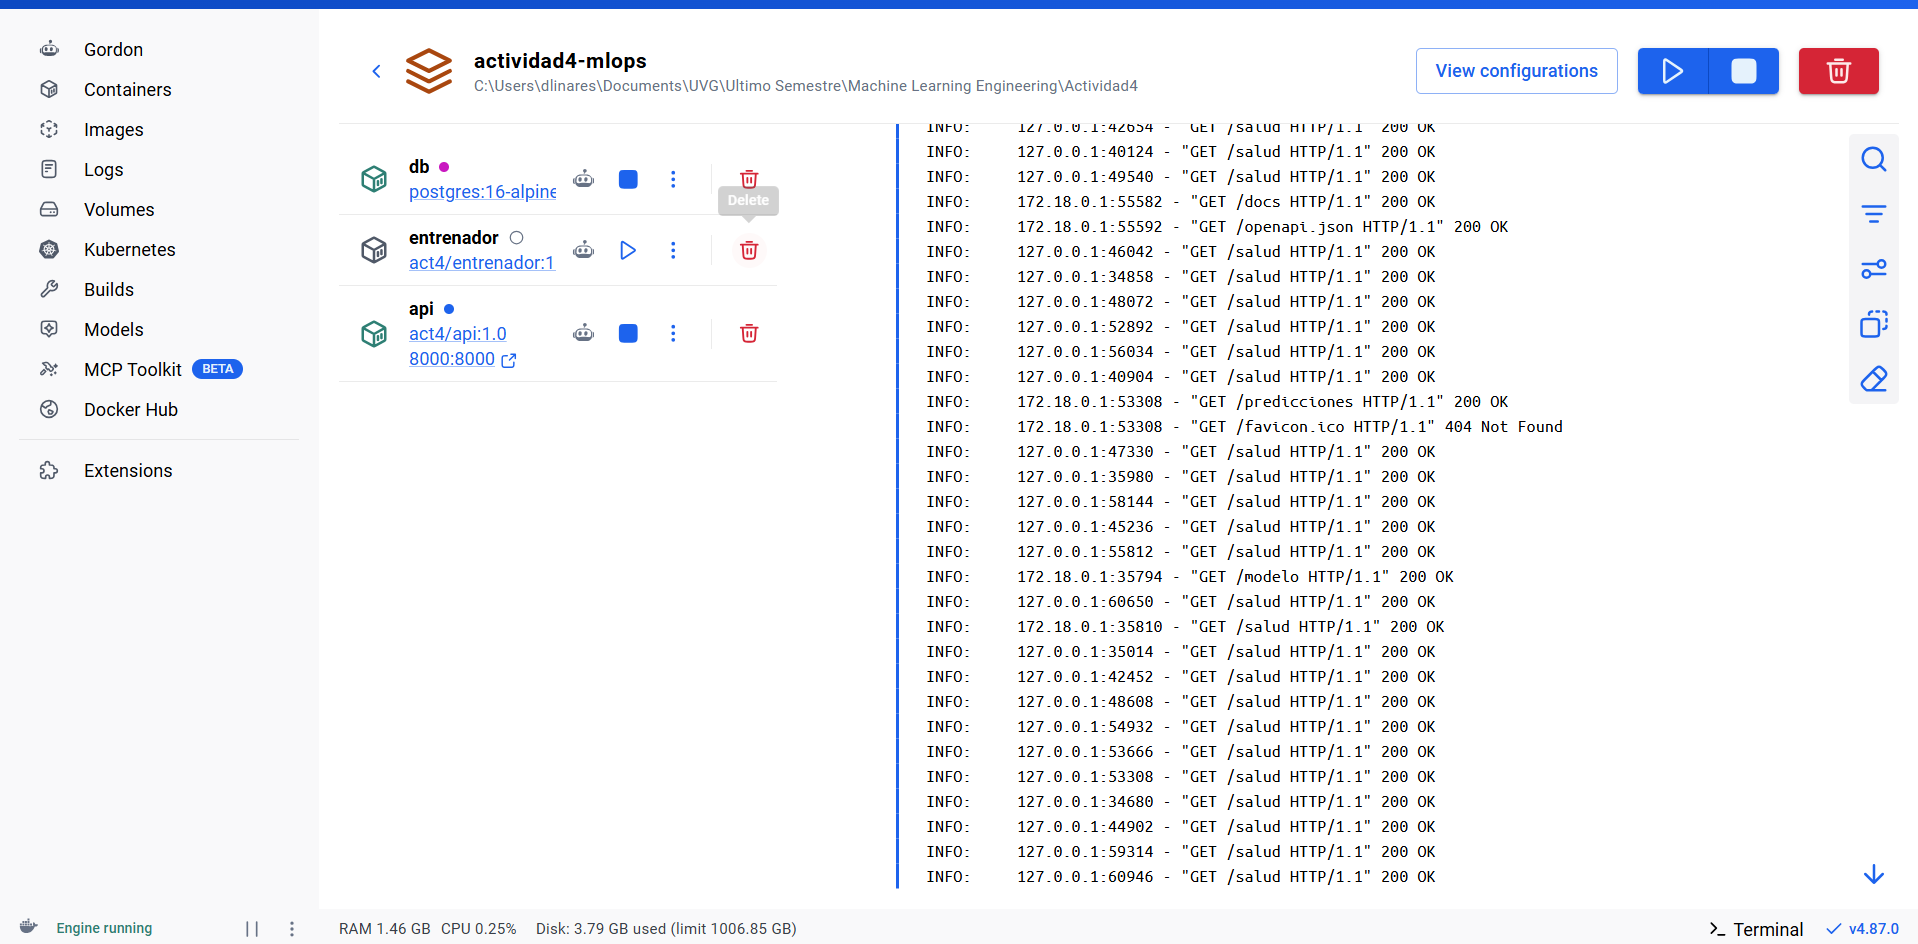
\includegraphics[width=\textwidth]{capturas/contenedorDocker.png}
\caption{Docker Desktop mostrando el conjunto \texttt{actividad4-mlops}. Los tres servicios con su
imagen correspondiente: \texttt{db} sobre \texttt{postgres:16-alpine} y \texttt{api} sobre
\texttt{act4/api:1.0} en ejecuci\'on con el puerto 8000 publicado, mientras que
\texttt{entrenador} aparece detenido. A la derecha, las peticiones HTTP atendidas.}
\end{figure}

\begin{figure}[ht]
\centering
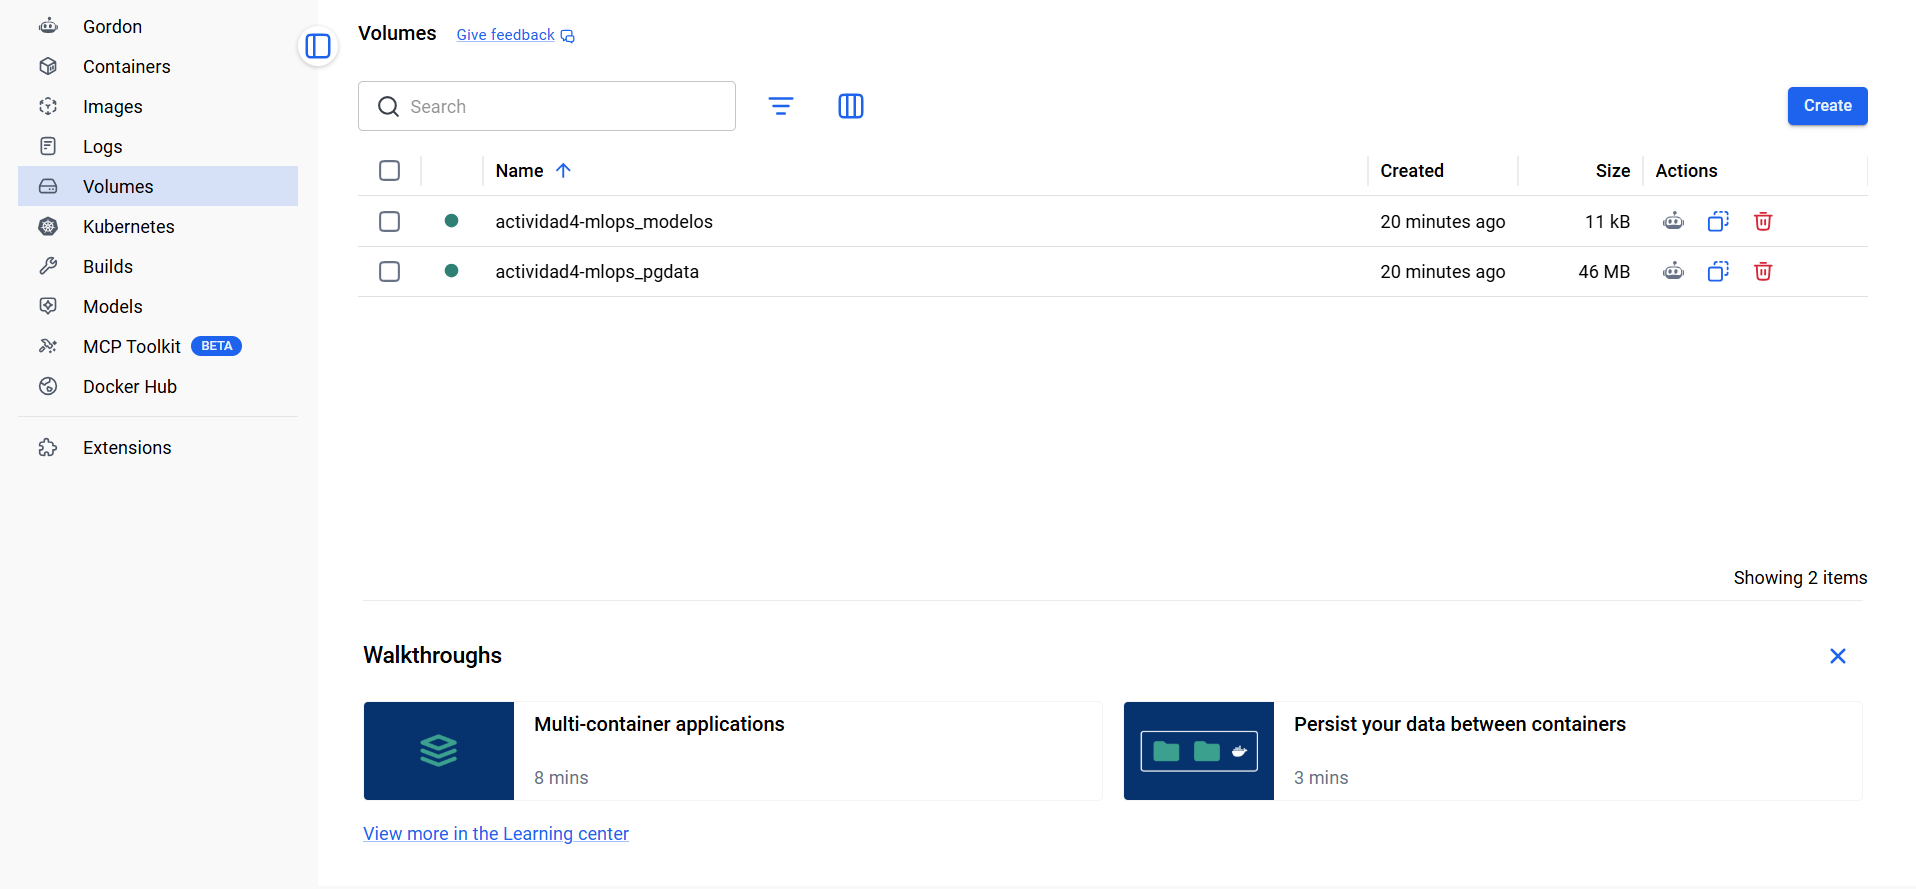
\includegraphics[width=\textwidth]{capturas/volumenesDocker.png}
\caption{Los vol\'umenes con nombre administrados por Docker: \texttt{actividad4-mlops\_modelos}
guarda el modelo entrenado y \texttt{actividad4-mlops\_pgdata} la base de datos. Existen de forma
independiente de los contenedores.}
\end{figure}

\begin{figure}[ht]
\centering
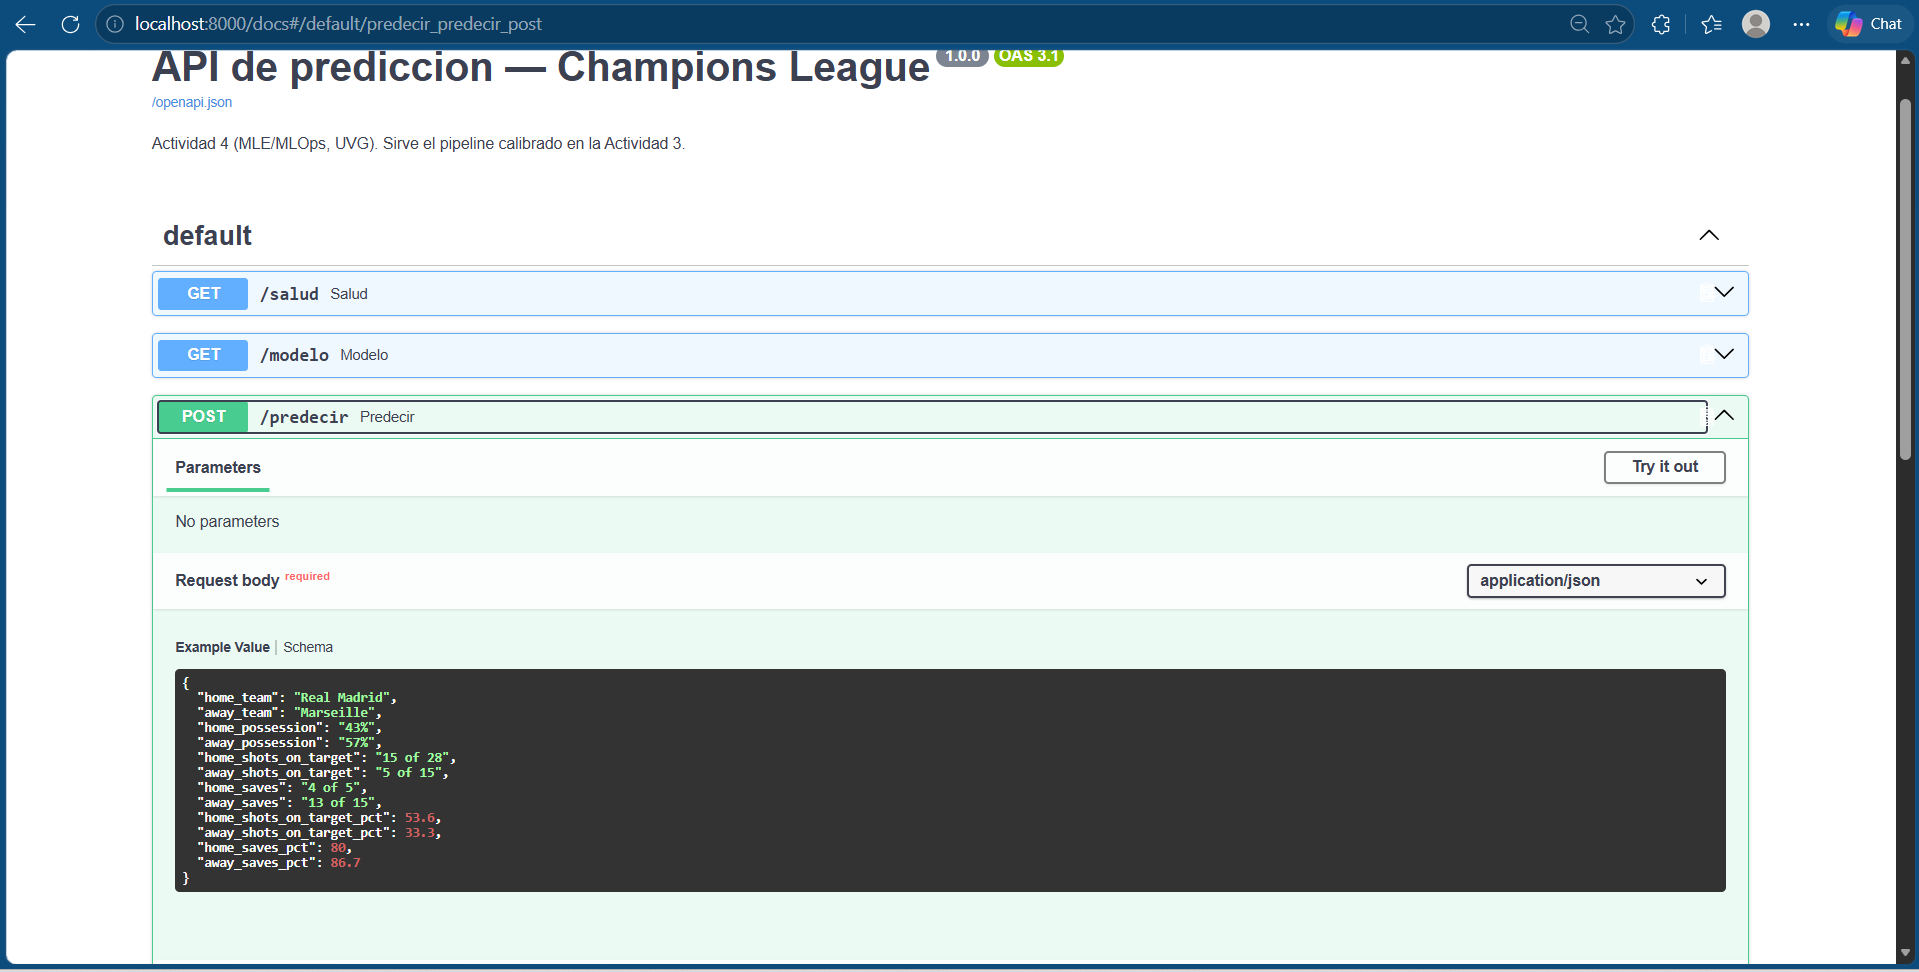
\includegraphics[width=\textwidth]{capturas/docsPredecir.png}
\caption{Documentaci\'on interactiva que FastAPI genera sola en \texttt{/docs}, con el endpoint
\texttt{POST /predecir} desplegado. El cuerpo de ejemplo muestra el formato que espera el
pipeline: la posesi\'on como texto (\texttt{"43\%"}) y los tiros como \texttt{"15 of 28"}, tal
como vienen en el CSV original.}
\end{figure}

\clearpage

\section{Conclusiones}

\begin{enumerate}
\item \textbf{Docker resuelve un problema que ya hab\'iamos sufrido.} La discrepancia de puntajes
entre Windows y macOS en la Actividad 3 se deb\'ia a versiones distintas de scikit-learn. Fijar
las versiones dentro de una imagen elimina esa clase completa de errores.

\item \textbf{El empaquetado de la Actividad 3 rindi\'o aqu\'i.} Ambas im\'agenes instalan el
mismo wheel, y no por comodidad: sin \'el, la API no podr\'ia reconstruir el pipeline serializado
porque no encontrar\'ia las clases de los transformadores propios.

\item \textbf{Separar el entrenamiento del servicio es la decisi\'on de arquitectura central},
porque ambas tareas tienen ritmos y requisitos opuestos: una es pesada y espor\'adica, la otra
liviana y constante.

\item \textbf{Sin vol\'umenes, un contenedor no recuerda nada.} El modelo y la base viven fuera
del ciclo de vida de los contenedores; los datos de entrada entran por bind mount. Cada tipo de
dato tiene su mecanismo y confundirlos se paga con p\'erdida de informaci\'on.

\item \textbf{Las condiciones de \texttt{depends\_on} sustituyen las esperas arbitrarias:} la API
arranca cuando el entrenador termin\'o correctamente y Postgres responde, no cuando transcurri\'o
un tiempo fijo.

\item \textbf{Correr sin privilegios exige preparar los vol\'umenes.} El \texttt{PermissionError}
que nos apareci\'o no fue un descuido aislado: es la consecuencia predecible de montar un volumen
vac\'io en un contenedor que no corre como \texttt{root}. Un volumen recuerda su propietario igual
que recuerda sus datos.
\end{enumerate}

\subsection*{Limitaciones y trabajo futuro}

El entrenador se ejecuta una \'unica vez al levantar el sistema; en producci\'on ser\'ia una tarea
programada o disparada por la llegada de datos nuevos. La API carga el modelo al arrancar, de modo
que un reentrenamiento exige reiniciarla. El modelo se guarda con un \'unico nombre, sin
versionado: un registro de modelos (por ejemplo MLflow) ser\'ia el siguiente paso natural. La
contrase\~na de la base viaja como variable de entorno, cuando lo correcto en producci\'on ser\'ia
usar \emph{secrets}. Finalmente, sigue vigente la limitaci\'on del modelo se\~nalada en la
Actividad 3: utiliza estad\'isticas que solo se conocen cuando el partido ya termin\'o, de manera
que explica el resultado m\'as de lo que lo predice.

\end{document}
